\documentclass[12pt,letterpaper]{article}
\usepackage{graphicx,textcomp}
\usepackage{natbib}
\usepackage{setspace}
\usepackage{fullpage}
\usepackage{color}
\usepackage[reqno]{amsmath}
\usepackage{amsthm}
\usepackage{fancyvrb}
\usepackage{amssymb,enumerate}
\usepackage[all]{xy}
\usepackage{endnotes}
\usepackage{lscape}
\newtheorem{com}{Comment}
\usepackage{float}
\usepackage{hyperref}
\newtheorem{lem} {Lemma}
\newtheorem{prop}{Proposition}
\newtheorem{thm}{Theorem}
\newtheorem{defn}{Definition}
\newtheorem{cor}{Corollary}
\newtheorem{obs}{Observation}
\usepackage[compact]{titlesec}
\usepackage{dcolumn}
\usepackage{tikz}
\usetikzlibrary{arrows}
\usepackage{multirow}
\usepackage{subcaption}
\usepackage{xcolor}
\newcolumntype{.}{D{.}{.}{-1}}
\newcolumntype{d}[1]{D{.}{.}{#1}}
\definecolor{light-gray}{gray}{0.65}
\usepackage{url}
\usepackage{listings}
\usepackage{color}

\definecolor{codegreen}{rgb}{0,0.6,0}
\definecolor{codegray}{rgb}{0.5,0.5,0.5}
\definecolor{codepurple}{rgb}{0.58,0,0.82}
\definecolor{backcolour}{rgb}{0.95,0.95,0.92}

\lstdefinestyle{mystyle}{
	backgroundcolor=\color{backcolour},   
	commentstyle=\color{codegreen},
	keywordstyle=\color{magenta},
	numberstyle=\tiny\color{codegray},
	stringstyle=\color{codepurple},
	basicstyle=\footnotesize,
	breakatwhitespace=false,         
	breaklines=true,                 
	captionpos=b,                    
	keepspaces=true,                 
	numbers=left,                    
	numbersep=5pt,                  
	showspaces=false,                
	showstringspaces=false,
	showtabs=false,                  
	tabsize=2
}
\lstset{style=mystyle}
\newcommand{\Sref}[1]{Section~\ref{#1}}
\newtheorem{hyp}{Hypothesis}

\title{Answer Key: Problem Set 1}
\date{Jeffrey Ziegler}
\author{Applied Stats/Quant Methods 1}

\begin{document}
	\maketitle
	
	\section*{Instructions}
\begin{itemize}
	\item \textit{Please show your work! You may lose points by simply writing in the answer. If the problem requires you to execute commands in \texttt{R}, please include the code you used to get your answers. Please also include the \texttt{.R} file that contains your code. If you are not sure if work needs to be shown for a particular problem, please ask.}
	\item \textit{Your homework should be submitted electronically on GitHub.}
	\item \textit{This problem set is due before 23:59 on Thursday October 9, 2025. No late assignments will be accepted.}

\end{itemize}

\vspace{1cm}
\section*{Question 1: Education}

\textit{A school counselor was curious about the average of IQ of the students in her school and took a random sample of 25 students' IQ scores. The following is the data set:}\\
\vspace{.25cm}

\lstinputlisting[language=R, firstline=40, lastline=40]{PS1_answerKey.R}  

\vspace{.5cm}

\begin{enumerate}
	\item \textit{Find a 90\% confidence interval for the average student IQ in the school.}\\
	
	
	\vspace{.15cm}
	\noindent First, let's calculate the t-score for the 90\% confidence interval with degrees of freedom equal to 24 (remember that df = $n-1$ for the t-distribution, and we're using the t-distribution because we have a small sample size). For the 90\% confidence interval, the lower tail is equal to 0.05 ($(1-\alpha)/2 = (1-0.90)/2 = 0.05$).\\
	
	\lstinputlisting[language=R, firstline=40, lastline=48]{PS1_answerKey.R}  
	
	\vspace{.15cm}
	\noindent Second, let's calculate the mean ($\bar{y}$),	the sample standard deviation $S$,  and then $\hat{\sigma}_{\bar{y}} = \displaystyle  \frac{S}{\sqrt{n}}$. This allows us to calculate our 90\% confidence interval for the student IQ as $\bar{y} \pm T \times \hat{\sigma}_{\bar{y}}$, which equals $98.44 \pm 1.71 \times \frac{13.09}{5}$ = [93.96, 102.92]. \\
	
	\lstinputlisting[language=R, firstline=50, lastline=56]{PS1_answerKey.R}  
	
	\vspace{.15cm}
	\noindent We can interpret this result by saying that if we took 100 samples, the true population mean of the student IQ in the school should fall within the interval in 90 of those samples.\\
	
	\item \textit{Next, the school counselor was curious  whether  the average student IQ in her school is higher than the average IQ score (100) among all the schools in the country.}\\ %She took a random sample of 25 students' IQ scores. 
	
	\noindent \textit{Using the same sample, conduct the appropriate hypothesis test with $\alpha=0.05$.}


\vspace{.5cm}

\noindent First, let's set up our null hypothesis: we want to know whether the mean of the sample ($\bar{y}$ or $\hat{\mu}$) is greater than the theoretical mean ($\mu_0$). So, using proof by contradiction, $H_0: \hat{\mu} \leq \mu_0$. Next, let's compute the standard error and our test statistic to get a p-value. Remember, since this is a one-sided test, we don't want both tails, so \texttt{lower.tail=F}.\\


\lstinputlisting[language=R, firstline=58, lastline=64]{PS1_answerKey.R}  
\vspace{.5cm}
\noindent We can see that the p-value ($\approx 0.72$) is not equal to or below the $\alpha=0.05$ threshold, so we would say that we do not find sufficient evidence to reject the null hypothesis that the average IQ of the students in this school is less than or equal to the population average IQ score ($\mu_0\leq$100). This makes sense; it's unlikely that we would have enough evidence to suggest that the average in the sample was larger than the population mean given that it is in fact lower.\\

\vspace{.15cm}
\noindent  We can also check our answer by using the \texttt{t.test} function in \texttt{R}. Note that if you only run this function and do not describe the steps of conducting a hypothesis test, that is not enough for full credit.\\

\lstinputlisting[language=R, firstline=65, lastline=66]{PS1_answerKey.R}  
\end{enumerate}

\vspace{.5cm}
	\section*{Question 2: Political Economy}

\noindent \emph{Researchers are curious about what affects the amount of money communities spend on addressing homelessness. The following variables constitute our data set about social welfare expenditures in the USA. } \\
\vspace{.5cm}

\begin{tabular}{r|l}
	\texttt{State} &\emph{50 states in US} \\
	\texttt{Y} & \emph{per capita expenditure on shelters/housing assistance in state}\\
	\texttt{X1} &\emph{per capita personal income in state} \\
	\texttt{X2} &  \emph{Number of residents per 100,000 that are "financially insecure" in state}\\
	\texttt{X3} &  \emph{Number of people per thousand residing in urban areas in state} \\
	\texttt{Region} &  \emph{1=Northeast, 2= North Central, 3= South, 4=West} \\
\end{tabular}

\vspace{.25cm}
\begin{itemize}
\item [(a)] \emph{Explore the \texttt{expenditure} data set and import data into \texttt{R}.}
\end{itemize}
\vspace{.5cm}
\lstinputlisting[language=R, firstline=72, lastline=75]{PS1_answerKey.R}  
\newpage

\begin{verbatim}
STATE          Y                X1             X2              X3       
AK     : 1   Min.   : 49.00   Min.   :1053   Min.   :334.0   Min.   :326.0  
AL     : 1   1st Qu.: 68.25   1st Qu.:1698   1st Qu.:374.2   1st Qu.:426.2  
AR     : 1   Median : 81.00   Median :1897   Median :395.0   Median :568.0  
AZ     : 1   Mean   : 85.04   Mean   :1912   Mean   :404.7   Mean   :561.7  
CA     : 1   3rd Qu.:102.00   3rd Qu.:2096   3rd Qu.:419.5   3rd Qu.:661.2  
CO     : 1   Max.   :142.00   Max.   :2817   Max.   :637.0   Max.   :899.0  
\end{verbatim}
\vspace{.5cm}

\begin{itemize}
\item [(b)] 
\emph{Please plot the relationships among \emph{Y}, \emph{X1}, \emph{X2}, and \emph{X3}? What are the correlations among them (you just need to describe the graph and the relationships among them)?}
%\vspace{.25cm}

\lstinputlisting[language=R, firstline=77, lastline=82]{PS1_answerKey.R}  
\vspace{.25cm}

\begin{figure}[h!]\centering

	\caption{\footnotesize Scatterplot of relationship between $Y, X_1, X_2$, and $X_3$.}
		\label{fig:plot_3b}
	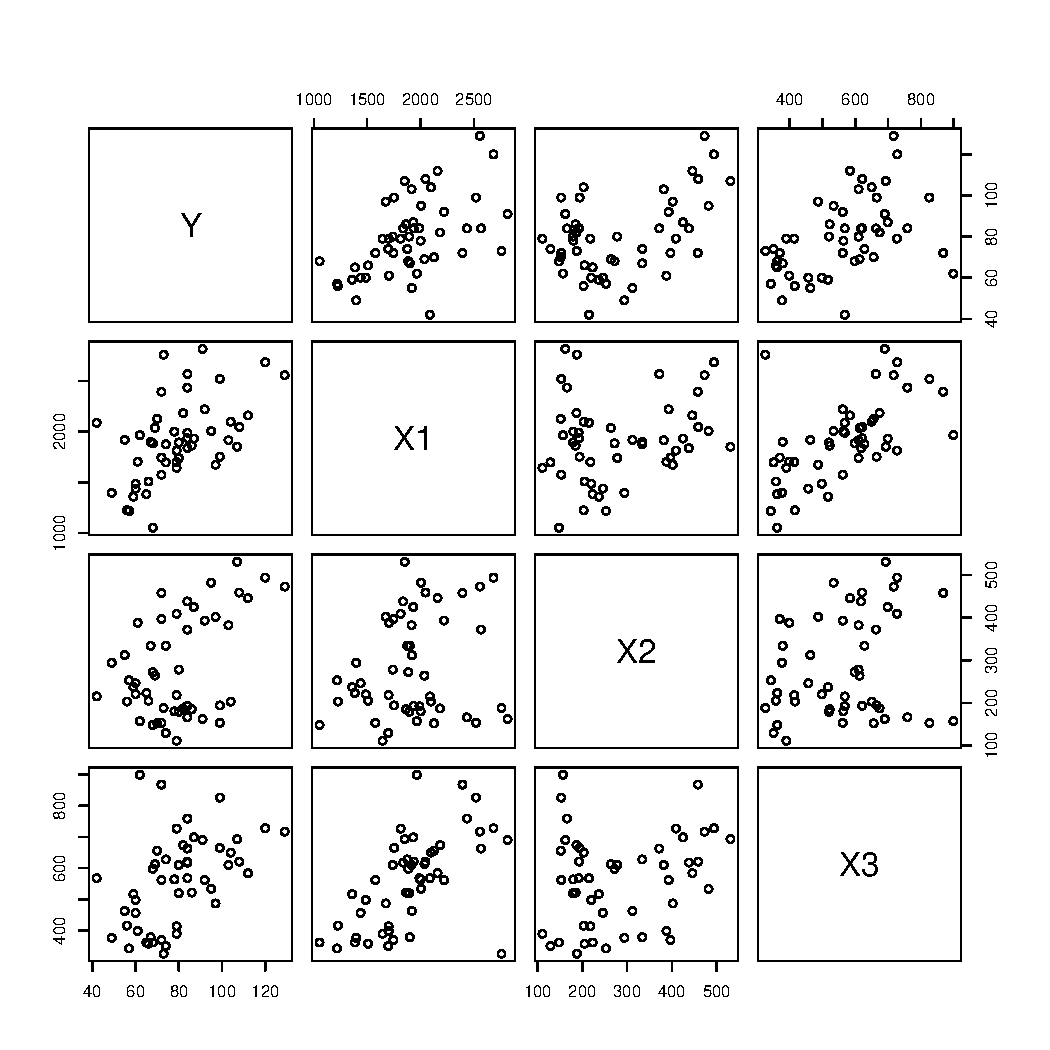
\includegraphics[width=.85\textwidth]{plot_2a.pdf}
\end{figure}

The correlation ($r$) between $Y$ and $X_1$ is 0.53, which indicates a moderate correlation and is consistent with the two subplots in the top-left of Figure~\ref{fig:plot_3b}. However, the correlation between $Y$ and $X2$, and $Y$ and $X3$, are weak (-0.21, 0.22).\\

We can also see that there is a positive relationship between $X_1$ and $X_3$, though there is not much of a relationship between $X_1$ and $X_2$, or $X_2$ and $X_3$. 

\vspace*{1cm}
\item [(c)]
\emph{Please plot the relationship between \emph{Y} and \emph{Region}? On average, which region has the highest per capita expenditure on public education?}

\vspace*{.5cm}

\lstinputlisting[language=R, firstline=84, lastline=87]{PS1_answerKey.R}  
%\vspace{.25cm}

\vspace*{.5cm}

\begin{figure}[h!]\centering
	\caption{\footnotesize Boxplot of $Y$ by $Region$.}\vspace{-1cm}
	\label{fig:plot_3c}
	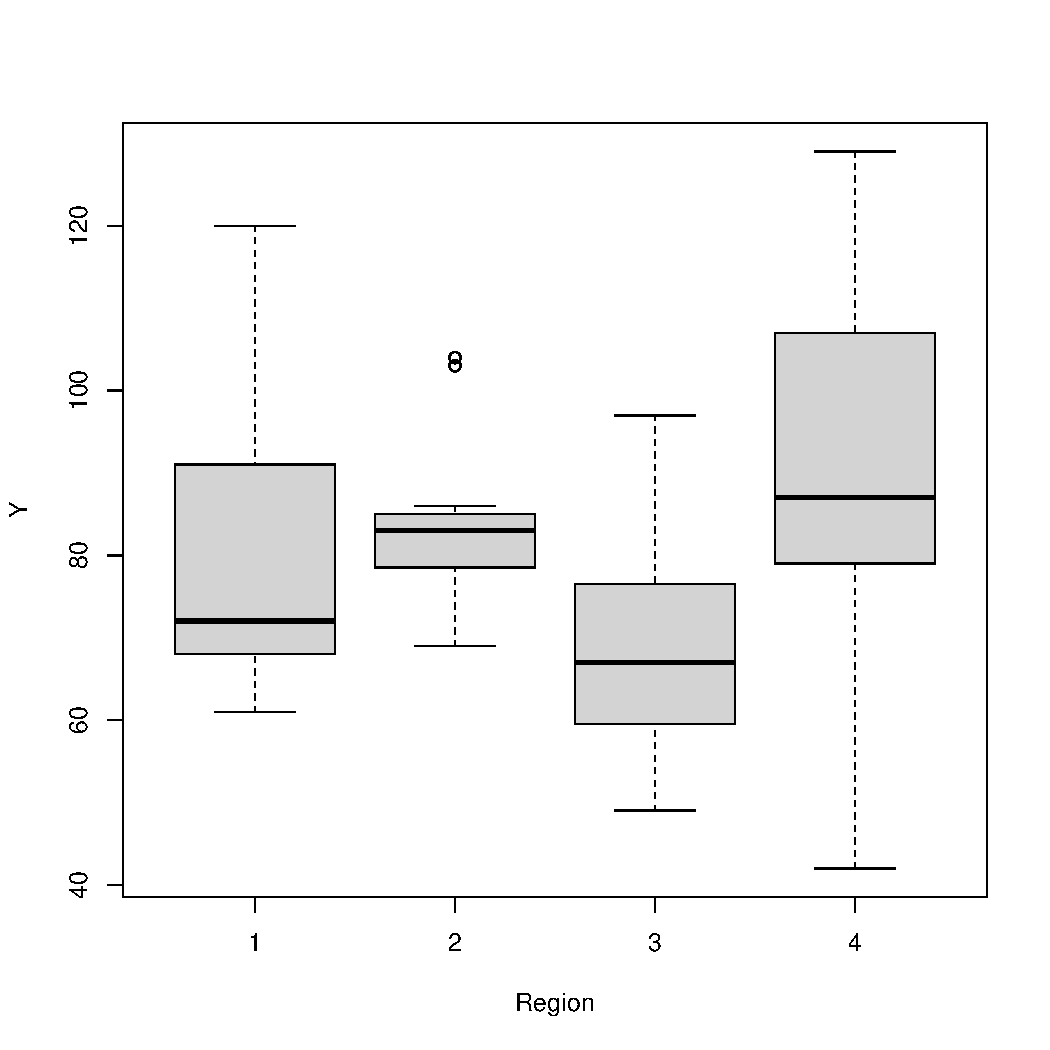
\includegraphics[width=.75\textwidth]{plot_2b.pdf}
\end{figure}

Figure~\ref{fig:plot_3c} displays the box-plot of $Y$ by $Region$ side-by-side, which is appropriate because $Region$ is a categorical variable and Y is a quantitative variable. The above code generates a side-by-side box-plot for the variables $Y$ and $Region$. From Figure~\ref{fig:plot_3c}, we can see that Region 4 has the highest per capita expenditure on public education.

\clearpage
\item [(d)] 
\emph{Please plot the relationship between \emph{Y} and \emph{X1}? Describe this graph and the relationship. Reproduce the above graph including one more variable \emph{Region} and display different regions with different types of symbols and colors.}
\end{itemize}
\vspace{.25cm}
\lstinputlisting[language=R, firstline=89, lastline=118]{PS1_answerKey.R}  

\begin{figure*}[h!]
	\centering
			\caption{\footnotesize Differentiating between region by color and shape.}
		\label{fig:plot3d}
	\begin{subfigure}[t]{0.5\textwidth}
		\centering
				\caption{\footnotesize Using base R.}
		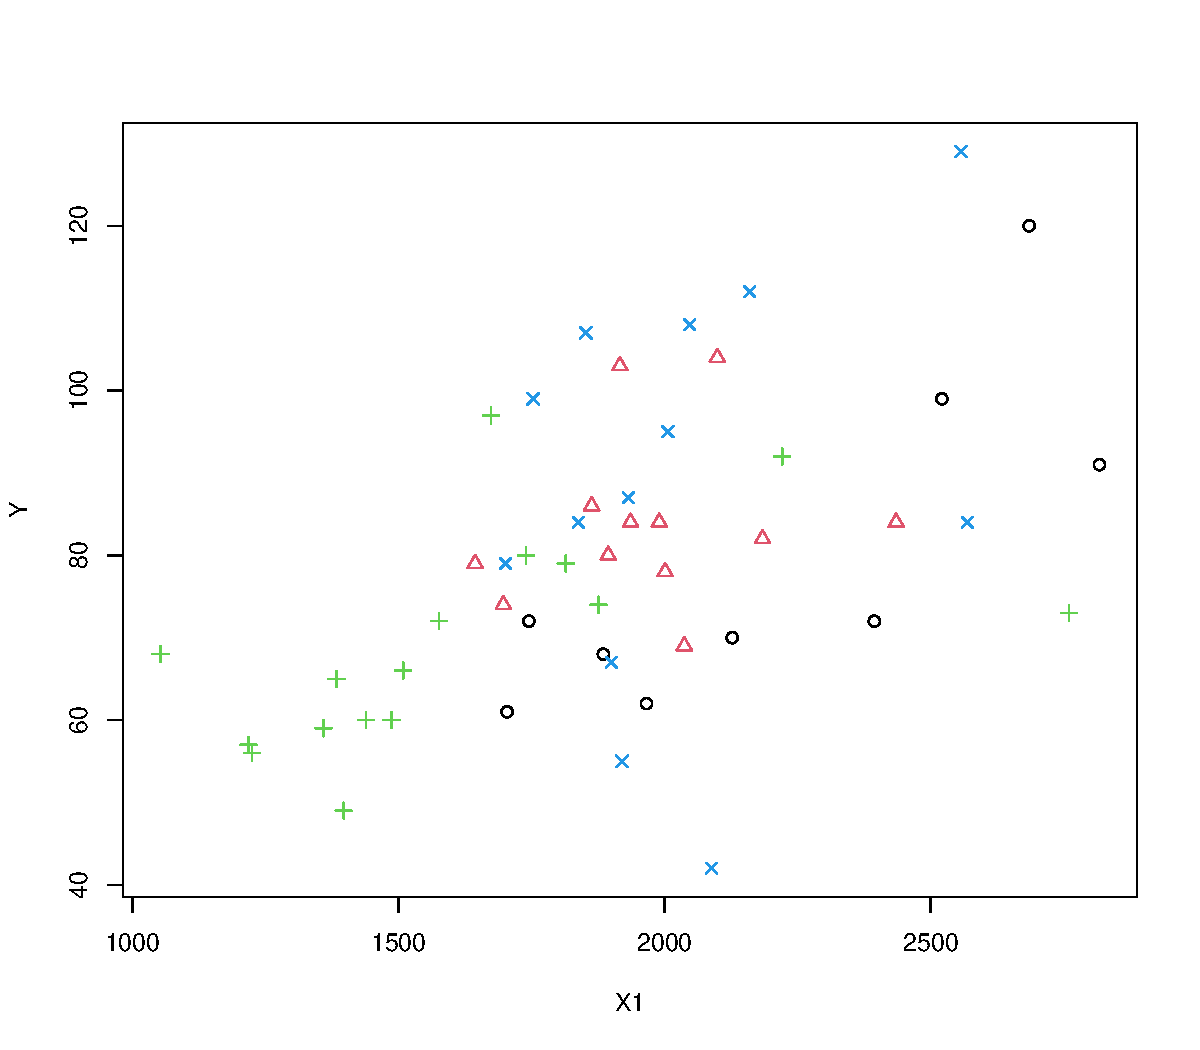
\includegraphics[width=0.99\textwidth]{plot_2c2.pdf}
	\end{subfigure}%
	\begin{subfigure}[t]{0.5\textwidth}
		\centering
			\caption{\footnotesize Using ggplot.}
		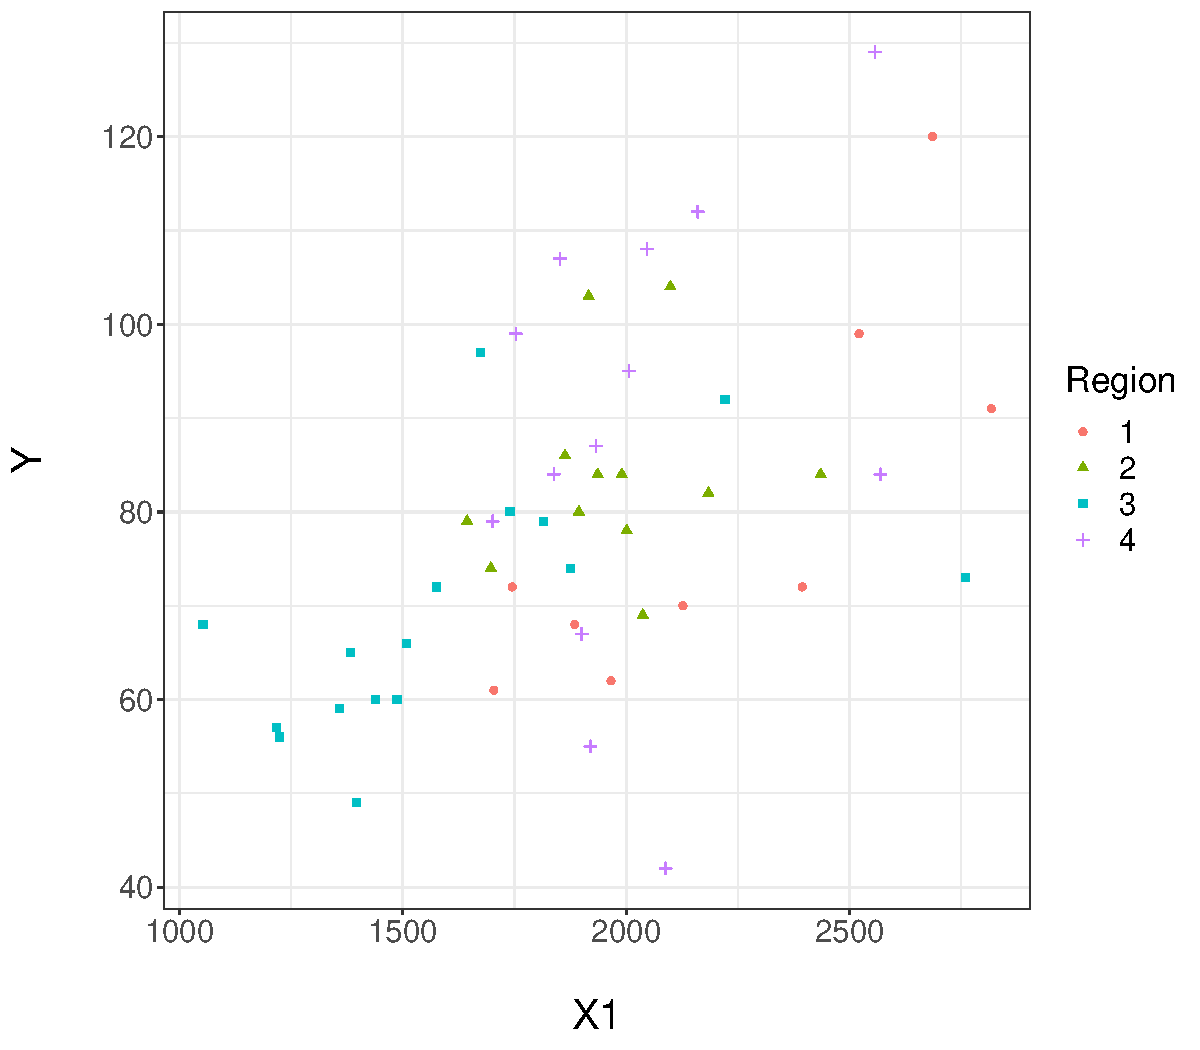
\includegraphics[width=0.99\textwidth]{plot_2c3.pdf}

	\end{subfigure}

\end{figure*}

\noindent We're using a scatter plot because both of these variables are quantitative, and we can see from Figure~\ref{fig:plot3d} that there is a moderate positive linear correlation between $X_1$ and $Y$ (which we noted in the above question). However, we can see in the right plot of Figure~\ref{fig:plot3d} that certain regions have much steeper (higher) or flatter (lower) correlations between $Y$ and $X_1$, which suggests that the effect of $X_1$ of $Y$ differs by region.

\end{document}
